\chapter{Izračun}


V tem poglavju bom s primerom dokazal, da program računa parametre pretočne hidroelektrarne pravilno. Za dokaz bom uporabil namišljen primer trapezno oblikovane struge vodotoka prikazane na sliki \ref{fig:izracun_trapeznaStruga} z Manningovim koeficientom hrapavosti 0,3 in z 1\% naklonom struge. Rezultate ročnega izračuna primerjal z rezultati ki jih izračuna program po trapezni metodi in numerični metodi opisani v poglavju \ref{sec:pretok_prav_trapez}  oz. \ref{sec:pretokNumericnaMetoda}.



\begin{figure}[ht!]
	\begin{centering}
		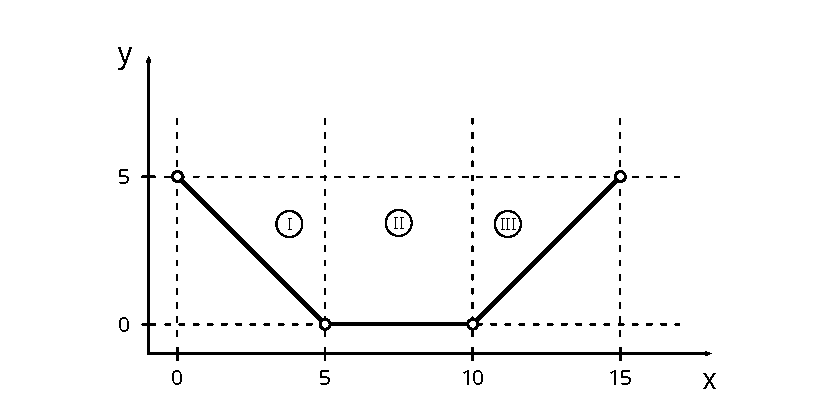
\includegraphics[width=\textwidth]{slike/izracuni/trapeznaStruga.pdf}		
		\caption{Struga vodotoka katerega bomo preračunali}\label{fig:izracun_trapeznaStruga}
	\end{centering}
\end{figure}

\section{Ročni izračun parametrov hidroelektrarne}

\begin{enumerate}[I.]
	
	\item Odsek
	
		\begin{align}
			S_I = \dfrac{5 * 5}{2} = 12,5
		\end{align}
		
		\begin{align}
			P_I = \sqrt{5^2 + 5^2} = 7,07
		\end{align}
		
		\begin{align}
			Q_1 = \dfrac{\sqrt{0,01}}{0,03} * \dfrac{12,5^{5/3}}{7,07^{2/3}} = 
		\end{align}
	
	
\end{enumerate}


aa


\section{Izračun parametrov hidroelektrarne s programom}

S pomočjo uporabniškega vmesnika v koordinatni sistem vnašamo serijo točk, ki predstavljajo robove izbrane struge. V tabeli na levi strani diagrama, za vsak odsek med dvema točkama dodajamo Manningove koeficiente hrapavosti $ng$ in naklone struge na sliki označene s $\varphi$. V našem primeru so vrednosti koeficientov za vse odseke rečne struge enake.

\begin{figure}[ht!]
	\begin{centering}
		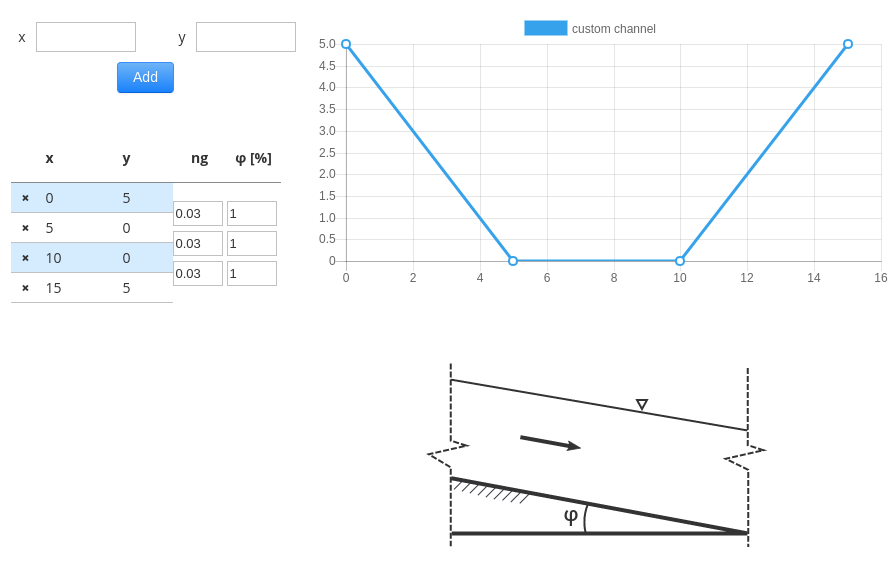
\includegraphics[width=\textwidth]{slike/izracuni/modeliranjeStruge.png}		
		\caption{Vnos podatkov v program}\label{fig:modeliranjeStruge}
	\end{centering}
\end{figure}
